
% This LaTeX was auto-generated from MATLAB code.
% To make changes, update the MATLAB code and republish this document.

\documentclass{article}
\usepackage{graphicx}
\usepackage{color}

\sloppy
\definecolor{lightgray}{gray}{0.5}
\setlength{\parindent}{0pt}

\begin{document}

    
    
\subsection*{Contents}

\begin{itemize}
\setlength{\itemsep}{-1ex}
   \item Part 1: Interpolation
   \item Part 3: Polynomial grid
   \item Part 4: Plotting
\end{itemize}
\begin{verbatim}
% Econ 527 Spring 2026 Question 2
% Professor Greaney
% Written by: Camille Bergeron
% Due: April 21, 2026
% Last Edited: April 17, 2026
\end{verbatim}


\subsection*{Part 1: Interpolation}

\begin{verbatim}
% vector for consumption grid
c_grid = linspace(0.1, 30, 100); % consumption grid from 0.1 to 30 with step of 0.01
disp('Consumption grid:');
disp(c_grid(1:10));

% evaluating utility function at the consumption grid points

% making CRRa utilty function
function u = crra_utility(c, gamma)
    if gamma == 1
        u = log(c); % logarithmic utility for gamma = 1
    else
        u = c.^(1-gamma) / (1-gamma); % CRRA utility for gamma != 1
    end
end

gamma = 4; % risk aversion parameter
u_grid = crra_utility(c_grid, gamma); % utility grid using CRRA utility function
disp('Original utility values:');
disp(u_grid(1:10));

% spline interpolation
spline_interp = spline(c_grid, u_grid); % create spline interpolation object
c_grid_interp = linspace(0.1, 30, 1000); % new consumption grid for interpolation
u_interp = ppval(spline_interp, c_grid_interp); % evaluate spline interpolation at new dense consumption grid

% calculating error at each grid point
u_original = crra_utility(c_grid_interp, gamma); % original utility values at the new dense grid
error = abs(u_original - u_interp); % absolute error between original and interpolated utility values
disp('Maximum error between original and interpolated utility values:');
disp(max(error));

% Plotting the original utility values and the interpolated values
figure;
fig = figure;
theme(fig, "light");
fplot(@(x) crra_utility(x, gamma), [0.1, 30], 'r-', 'DisplayName', 'Original Utility', LineWidth=2); % original utility function
hold on;
plot(c_grid_interp, u_interp, 'b-', 'DisplayName', 'Spline Interpolation', LineWidth=2); % spline interpolation
xlabel('Consumption');
ylabel('Utility');
title('Utility Function and Spline Interpolation');
legend;
grid on;
saveas(gcf,'./figs/spline_interpolation.fig')
saveas(gcf,'./figs/spline_interpolation.png')
\end{verbatim}

        \color{lightgray} \begin{verbatim}Consumption grid:
  Columns 1 through 7

    0.1000    0.4020    0.7040    1.0061    1.3081    1.6101    1.9121

  Columns 8 through 10

    2.2141    2.5162    2.8182

Original utility values:
  Columns 1 through 7

 -333.3333   -5.1302   -0.9552   -0.3273   -0.1489   -0.0799   -0.0477

  Columns 8 through 10

   -0.0307   -0.0209   -0.0149

Maximum error between original and interpolated utility values:
  141.5997

\end{verbatim} \color{black}
    

\includegraphics [width=4in]{PS1_Q2_01.eps}

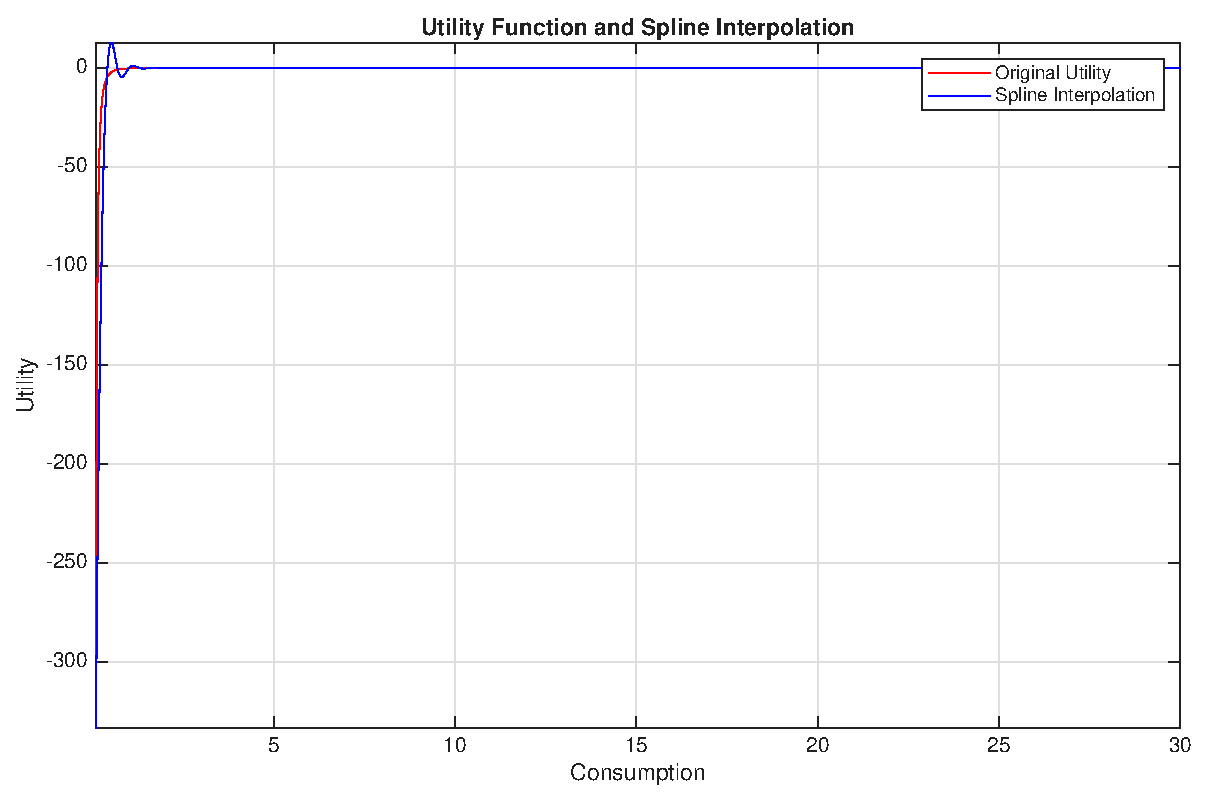
\includegraphics [width=4in]{PS1_Q2_02.eps}


\subsection*{Part 3: Polynomial grid}

\begin{verbatim}
% function to create polynomial grid
function c_grid_poly = polynomial_grid(point_a, point_b, nodes, curve)
    c_grid_normalized = linspace(0, 1, nodes); % normalized grid in [0,1]
    c_grid_poly = point_a + (point_b - point_a) * c_grid_normalized.^curve; % polynomial transformation
end

% creating polynomilial grid for consumption
curve = 3; % curvature parameter for polynomial grid
c_grid_poly = polynomial_grid(0.1, 30, 1000, curve); % polynomial grid transformation
disp('Polynomial consumption grid:');
disp(c_grid_poly(1:10));

u_grid_poly = crra_utility(c_grid_poly, gamma); % utility grid using CRRA utility function
disp('Original utility values:');
disp(u_grid_poly(1:10));

% spline interpolation, again
spline_interp_poly = spline(c_grid_poly, u_grid_poly); % create spline interpolation object
c_grid_interp_poly = linspace(0.1, 30, 1000); % new consumption grid for interpolation
u_interp_poly = ppval(spline_interp_poly, c_grid_interp_poly); % evaluate spline interpolation at new dense consumption grid

% calculating error at each grid point
u_original_poly = crra_utility(c_grid_interp_poly, gamma); % original utility values at the new dense grid
error_poly = abs(u_original_poly - u_interp_poly); % absolute error between original and interpolated utility values
disp('Maximum error between original and interpolated utility values:');
disp(max(error_poly));
\end{verbatim}

        \color{lightgray} \begin{verbatim}Polynomial consumption grid:
  Columns 1 through 7

    0.1000    0.1000    0.1000    0.1000    0.1000    0.1000    0.1000

  Columns 8 through 10

    0.1000    0.1000    0.1000

Original utility values:
  Columns 1 through 7

 -333.3333 -333.3330 -333.3309 -333.3252 -333.3141 -333.2958 -333.2686

  Columns 8 through 10

 -333.2305 -333.1798 -333.1148

Maximum error between original and interpolated utility values:
   2.8892e-07

\end{verbatim} \color{black}
    

\subsection*{Part 4: Plotting}

\begin{verbatim}
% making new consumption grid to plot, with 100 nodes
c_grid_plot = linspace(30, 40, 100); % new consumption grid for plotting
u_grid_plot = crra_utility(c_grid_plot, gamma); % original utility values at the new grid for plotting
u_interp_plot = ppval(spline_interp_poly, c_grid_plot); % interpolated utility

% Plotting the original utility values and the new interpolated values
figure;
fig = figure;
theme(fig, "light");
fplot(@(x) crra_utility(x, gamma), [30, 40], 'r-', 'DisplayName', 'Original Utility', LineWidth=3); % original utility function
hold on;
plot(c_grid_plot, u_interp_plot, 'b-', ...
    'DisplayName', 'Spline Interpolation Polynomial', Color='#DC94FF', LineWidth=3); % spline interpolation
xlim([30 40])
xlabel('Consumption');
ylabel('Utility');
title('Utility Function and Spline Interpolation with Polynomial Grid, 30-40');
legend;
grid on;
saveas(gcf,'./figs/spline_interpolation_poly_30-40.png')
saveas(gcf,'./figs/spline_interpolation_poly_30-40.fig')


% making new gridpoint
c_grid_plot = linspace(0.01, 0.1, 100); % new consumption grid for plotting
u_grid_plot = crra_utility(c_grid_plot, gamma); % original utility values at the new grid for plotting
u_interp_plot = ppval(spline_interp_poly, c_grid_plot); % interpolated utility values at the new grid for plotting


% Plotting the original utility values and the new interpolated values
figure;
fig = figure;
theme(fig, "light");
fplot(@(x) crra_utility(x, gamma), [0.01, 0.1], 'r-', 'DisplayName', 'Original Utility', LineWidth=3); % original utility function
hold on;
plot(c_grid_plot, u_interp_plot, 'b-', ...
    'DisplayName', 'Spline Interpolation Polynomial', Color='#DC94FF', LineWidth=3); % spline interpolation
xlim([0.01 0.1])
xlabel('Consumption');
ylabel('Utility');
title('Utility Function and Spline Interpolation with Polynomial Grid, 0.01-0.1');
legend;
grid on;
saveas(gcf,'./figs/spline_interpolation_poly_0.01-0.1.png')
saveas(gcf,'./figs/spline_interpolation_poly_0.01-0.1.fig')
\end{verbatim}

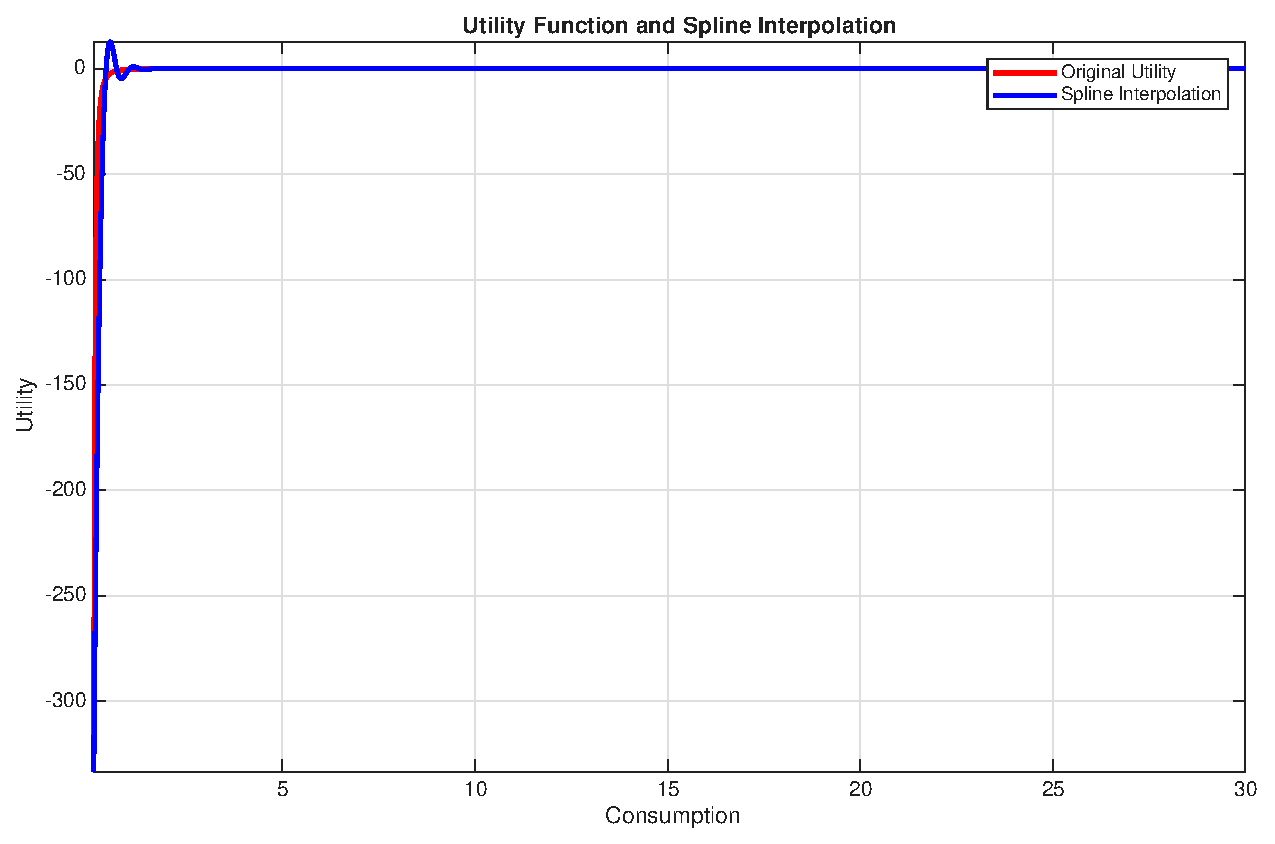
\includegraphics [width=4in]{PS1_Q2_03.eps}


\includegraphics [width=4in]{PS1_Q2_04.eps}

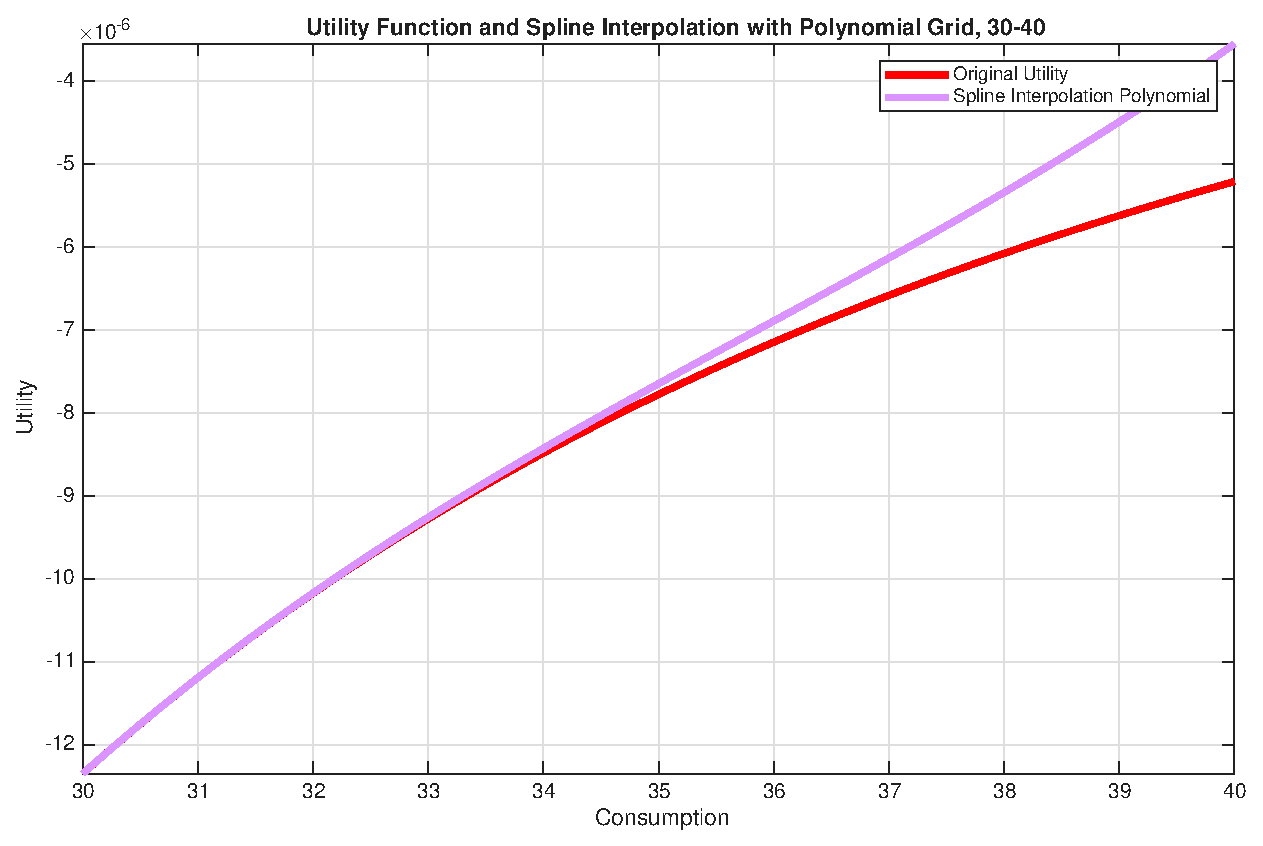
\includegraphics [width=4in]{PS1_Q2_05.eps}


\includegraphics [width=4in]{PS1_Q2_06.eps}

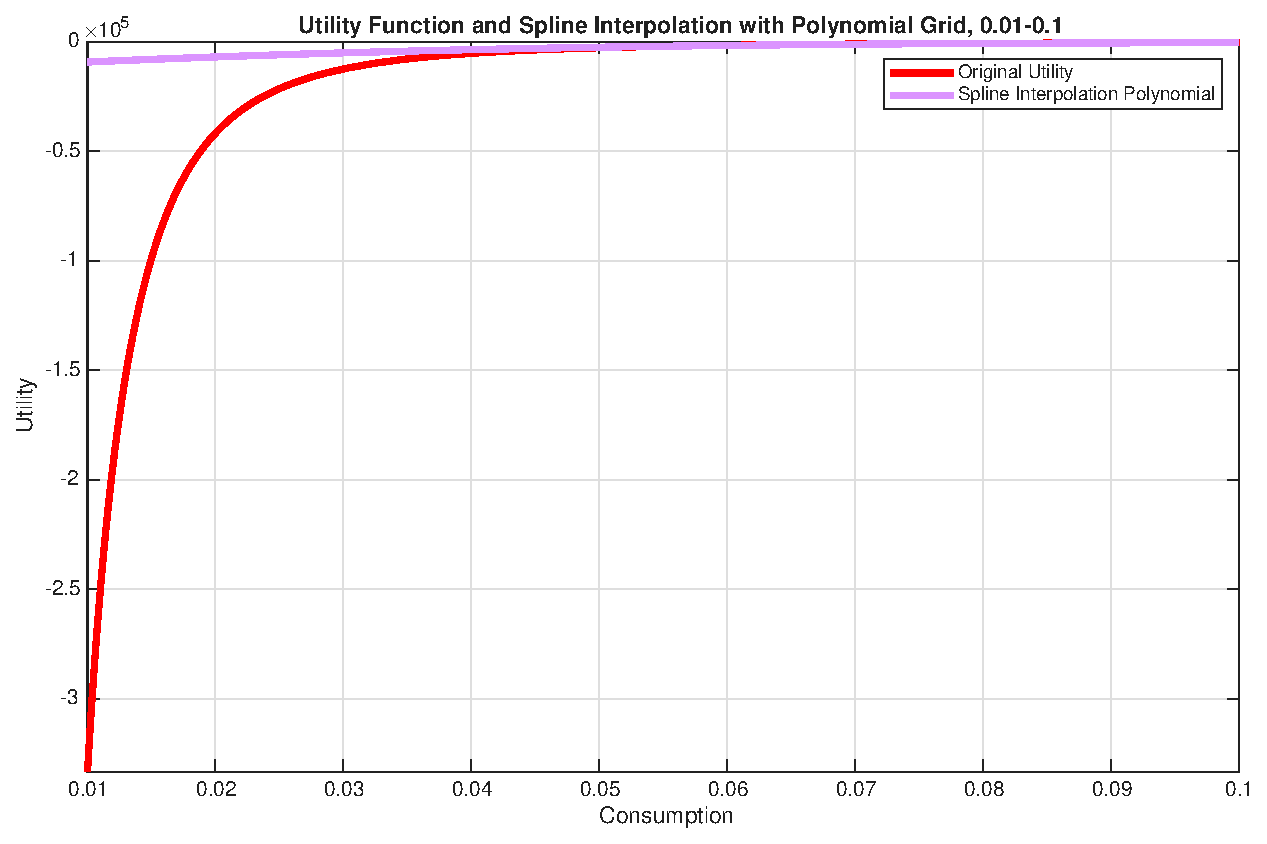
\includegraphics [width=4in]{PS1_Q2_07.eps}



\end{document}

